\subsection{Analisi}
Questa fase comincia con la presentazione dei capitolati d'appalto e termina con la data di consegna per la \textit{Revisione dei Requisiti}, ovvero dal 05-11-2020 al 11-01-2021.
In questo periodo verranno redatti tutti i documenti necessari e verrà fatta un'analisi approfondita del capitolato scelto dal gruppo \Gruppo{}.

\subsubsection{Obiettivi}
Organizzazione interna del team e stesura di tutti i documenti.

\subsubsection{Periodi e attività}
La pianificazione di questa fase è stata organizzata nei seguenti periodi:
\begin{itemize}
\item \textit{Dal 05-11-2020 al 04-12-2020}: individuazione degli strumenti per la comunicazione interna e discussione dei capitolati proposti. Inizio della stesura dello \SdF{} con \glo{milestone} il 10-12-2020;

\item \textit{Dal 05-12-2020 al 22-12-2020}: stesura delle \NdP{} e del \PdP{} e iniziata inoltre la stesura dell'\AdR{}. Il 22-12-2020 il gruppo ha fissato una milestone\glo{} per la verifica dei prodotti;

\item \textit{Dal 23-12-2020 al 05-01-2021}: il gruppo si dedica all'\AdR{} e al contempo inizia la stesura del \PdQ{}. Il 05-01-2020 il gruppo fissa un'ulteriore milestone\glo{} per verificare che tutti i documenti siano stati completati correttamente;

\item \textit{Dal 06-01-2021 al 11-01-2021}: si svolge attività di verifica su tutti i documenti, si completano eventualmente documenti in ritardo. Si uniformano tutti i documenti stando alle regole stabilite nelle \NdP{}.
\end{itemize}

\begin{landscape}

\begin{figure}[h]
	\centering
	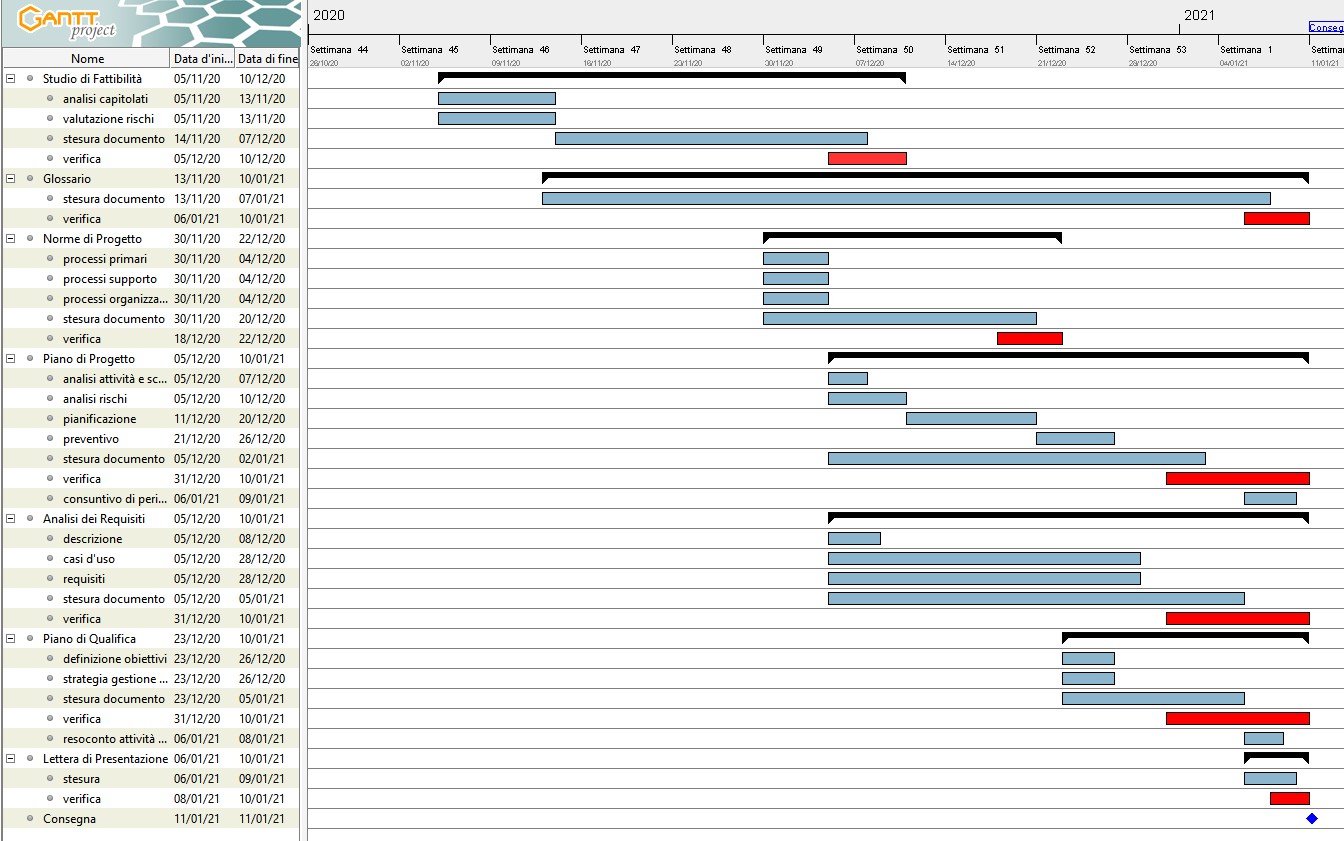
\includegraphics[width=\linewidth]{Images/GanttPianificazioneAnalisi.PNG}
	\caption{Diagramma di Gantt dell'attività di analisi}
\end{figure}

\end{landscape}



